
The DESY-type beam telescope are a tabletop trackers featuring six pixel detectors on aluminium rails, a Trigger and Logic Unit (TLU) providing trigger logic and time stamp information on particle passage,
 four scintillators with photo multiplier tubes (PMT) for trigger purposes, and hardware for the data read-out. 
Figure\,\ref{fig:datura-tscope} shows the sensor jigs, wherein the pixel sensors are embedded, with its auxiliary boards providing connections for power, JTAG-ing, clock signals, and data transmission.
A DUT is usually inserted in middle of the six planes, with three planes up- and down-stream of the DUT. 
In the chosen coordinate system, the XY plane is parallel to the sensor planes, with the X direction point horizontically, and Z points along the beam direction. 
 
\subsection{Sensors and mechanics}

The Mimosa26 detectors used for precise spacial measurement of particle trajectories are manufactured with the 350\,nm CMOS technology. 
Each Mimosa26 detector consist of pixels sized $\unit{18.4}{\upmu\meter} \times \unit{18.4}{\upmu\meter}$, which are arranged in 1152 columns and 576 rows.\,\cite{Mimosa26}
This adds to a total of about four million readout channels covering an area of roughly $\unit{10}{\milli\meter} \times \unit{20}{\milli\meter}$. 
The Mimosa26 sensors are $\unit{50}{\upmu\meter}$ thick and are protected on each side by $\unit{25}{\upmu\meter}$ thick, lightproof Kapton foil. 
A simple two transistors/one diode approach to collect diffused charge produced in the underlying \unit{14}{\upmu\meter} epitaxial layer
 allows the construction of small size pixels as in the case of Mimosa26 sensor.
The binary resolution of 18.4\,um pitch sensor is $\unit{18.4}{\upmu\meter}$, but charge charging improves the resolution as will be shown in Section~\ref{sec:trackres}.
%With the rising industrial interest in high resistivity epitaxial silicon for CMOS detectors the production cost of improved noise and radiation hardness parameters
% became already possible with ~400 Ohm·cm for 10 μm epitaxial layer for Mimosa26. 

The readout of the Mimosa26 detectors is performed in a rolling shutter approach, which takes 16 cycles of an 80 MHz clock per row, with all 1152 columns being readout in parallel. 
The 16 clock cycles allow for correlated double sampling and zero suppression being performed on-chip with the digital circuitry placed outside of the pixel array.
At this clock frequency the Mimosa26 integration time equals $\unit{115.2}{\upmu\second}$ and allows about 8680 frames per second to be read out. 
With the on-chip buffer size being able to accommodate the data of about a few hundred pixels (above threshold) on the sensor,
the expected maximum rate of particles through the active area estimates to about $\unit{1}{\mega\hertz/\centi\meter^2}$. 
The average noise occupancy per read-out frame is measured to be smaller than $2\cdot10^{-5}$ for non-irradiated sensors at room temperature at the signal-to-noise threshold level of six,
 consistent with an average efficiency of 99\,\%. 

Every pixel sensor is mounted within a aluminium jigs, and three jigs are in turn mounted on each of the two aluminium arms. 
Holes are machined in the jigs were the sensors sit, and hence the beam passes through, in order to minimise material budget. 
In total, this leads to a material budget of $\unit{300}{\upmu\meter}$ silicon and $\unit{300}{\upmu\meter}$ Kapton, which needs to be taken into account for electron/positron beams in the few GeV range. 
Each arm, one upstream and one downstream of the DUT, is adjustable in the beam direction in order to ease measurements varying in DUT size.
The minimal distance between two jigs is given by the jig thickness of 20\,mm, the maximal distance between two neighbouring jigs at equidistant spacing can be incresed to 150\,mm.
Furthermore, for stable performance each jig provides a colling inlet and putlet in order to keep the Mimosa26 sensors at a stable temperature. 
The entire tracker is placed on a rotatable frame easing the orientation parallel to the beam direction. 
Additionally, this frame is mounted on a sturdy structure providing stability over time and wheels for easy transportation. 

\begin{figure}[tb]
	\center
	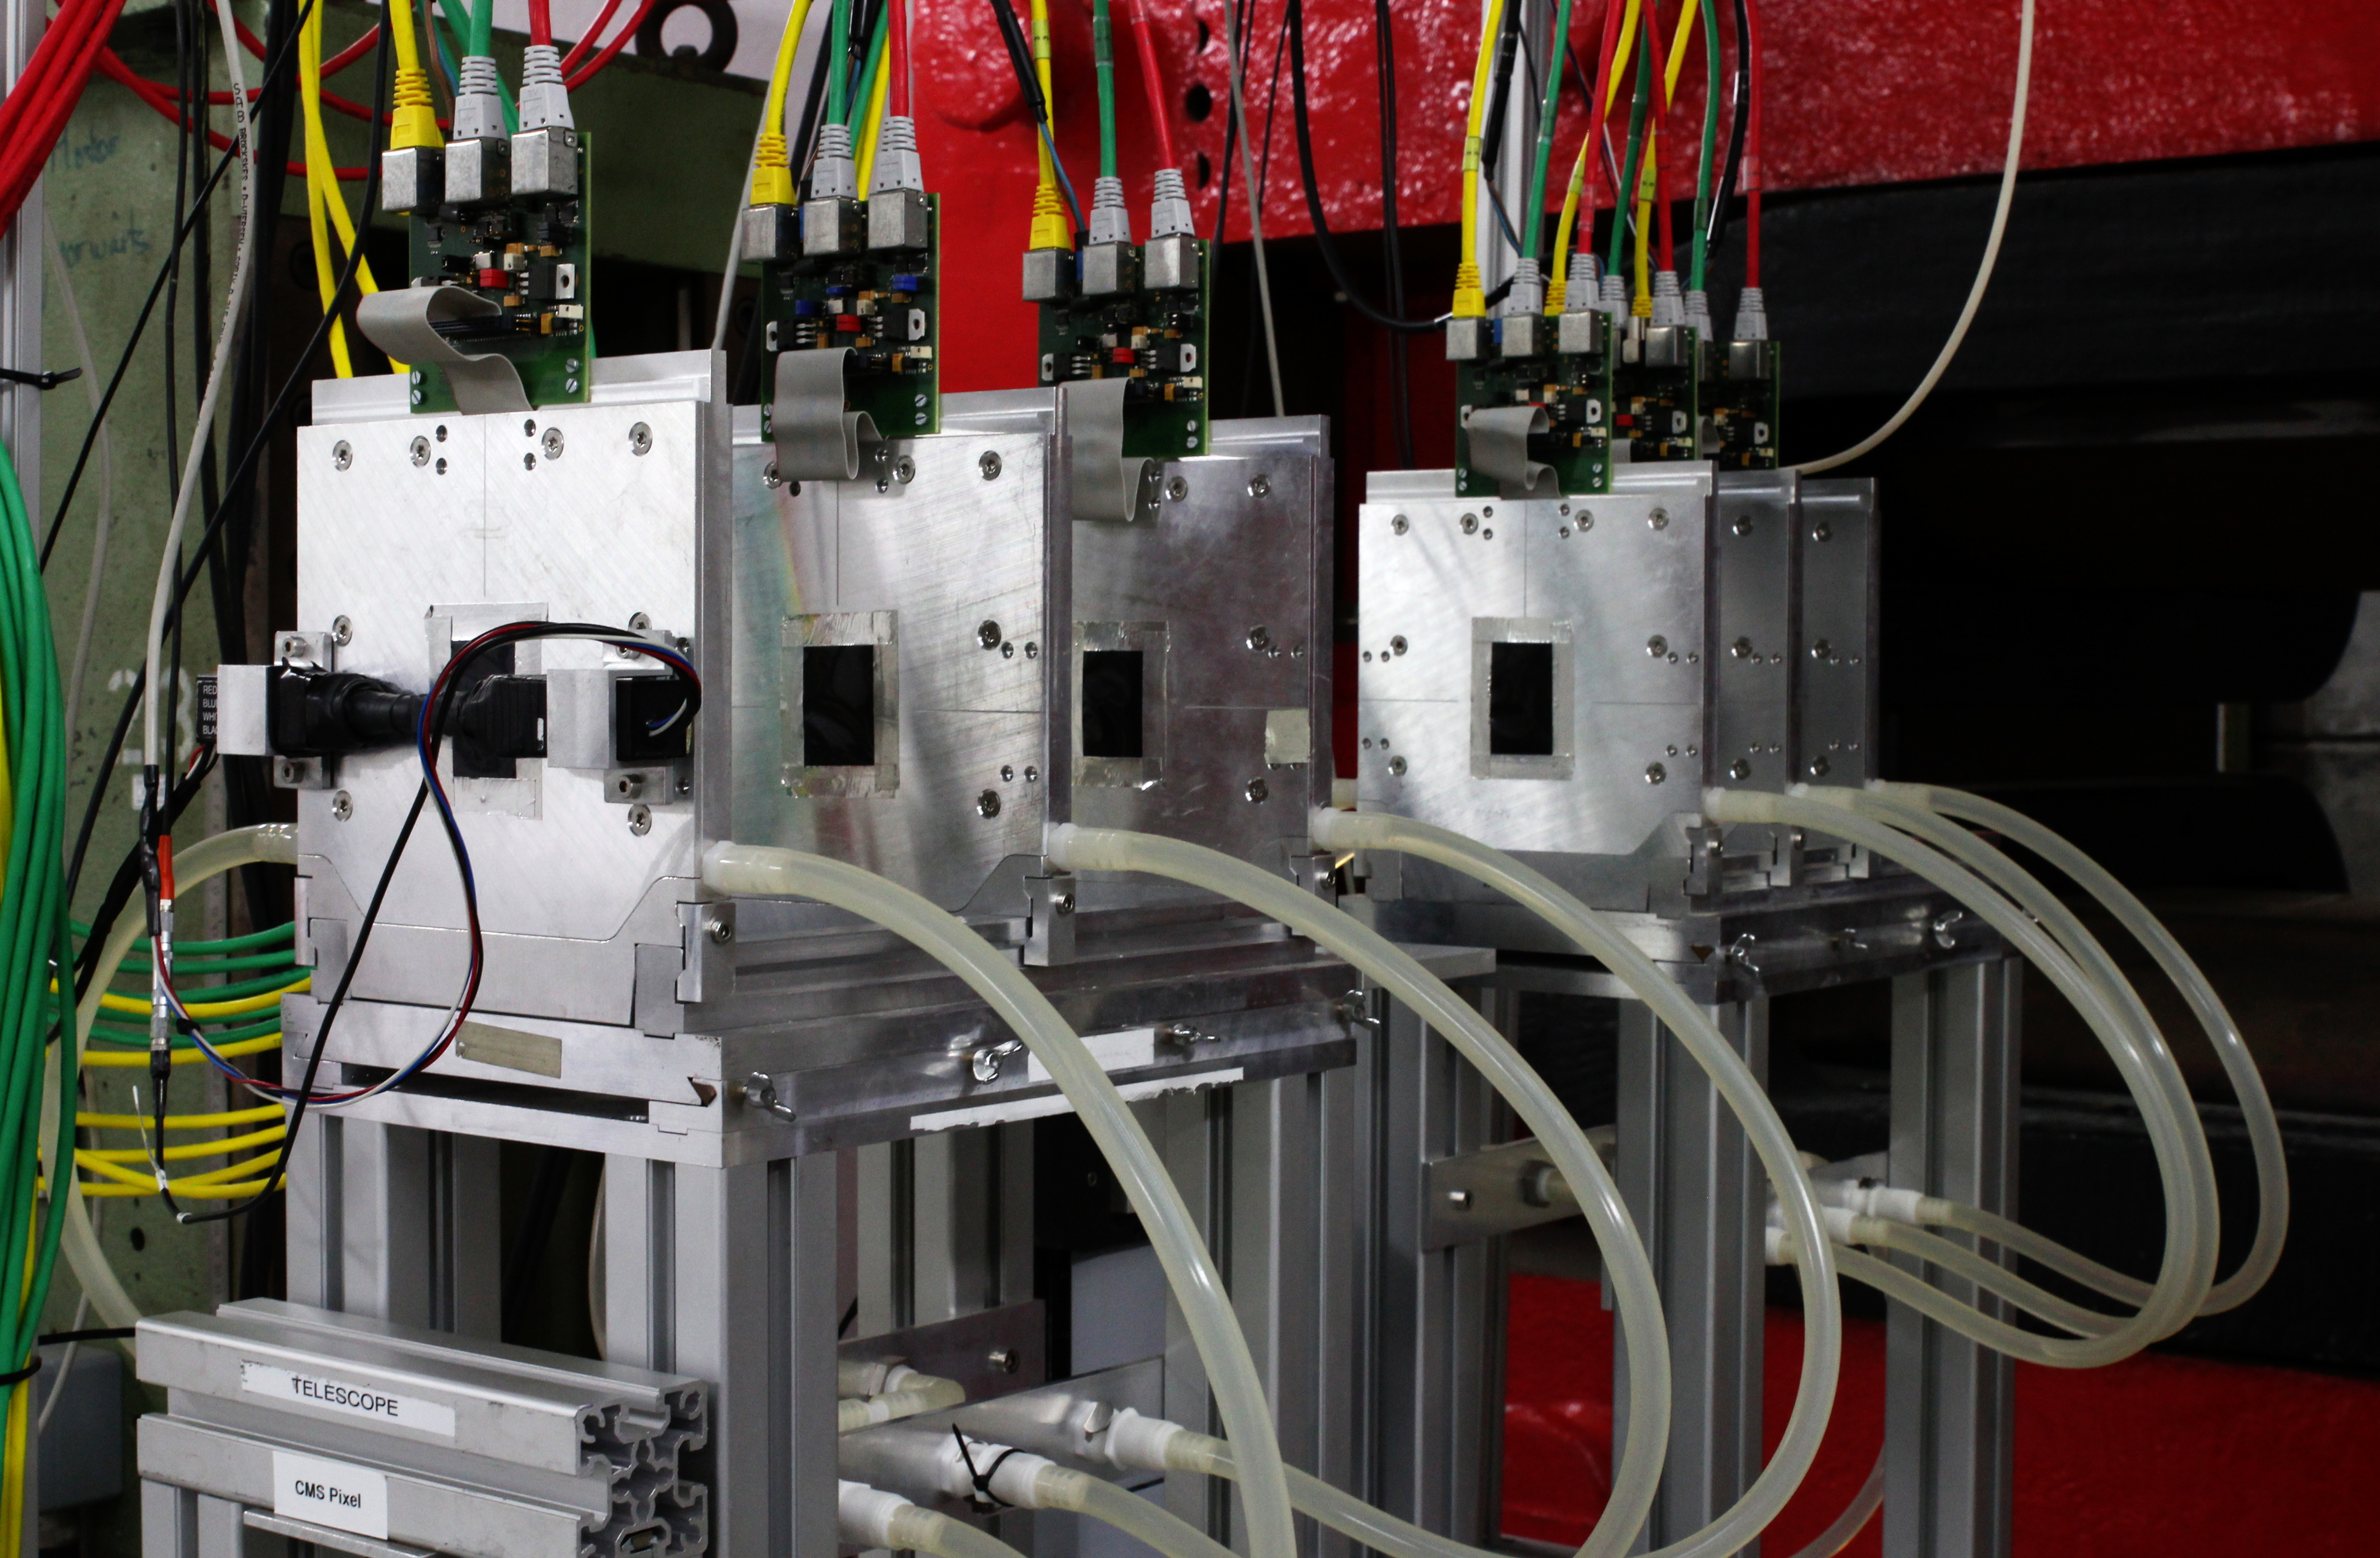
\includegraphics[width=.9\textwidth]{figures/DATURA.jpg}
	\caption[The \Datura telescope]{The \Datura telescope with its six Mimosa26 sensors on an aluminium rail is shown.}
	\label{fig:datura-tscope}
\end{figure}

\subsection{Trigger and DAQ system}

Four Hamamatsu PMTs assemblies with scintillators and lightguides, two in front and two in the back of the telescope, define the spatial acceptance window for triggers. 
The cross configuration of the scintillators define a rectangular acceptance window of 10\,mm times 20\,mm matching the Mimosa26 acceptance area. 
Additionally, a XY$\upphi$-stage is available for translation over the acceptance region and rotation of the DUT. 
Up to four PMT signals can be used to feed the TLU. 
Based on a commercial Spartan\,3 board, the TLU is equipped with several custom-made add-on PCBs in order to interface PMT input signals
 and integrate user DAQ systems in order to read-out devices under test like e.g.~LHC-type sensors. 
Providing a programmable logic, the TLU  takes a trigger decision and distributes the trigger signal to all DAQ systems integrated with the telescope framework.

From a hardware point of view, the Mimosa26 sensors provide the spatial, zero-suppressed hit data over a flat ribbon cable to the auxiliary boards, which provide RJ\,45 connectors to connect them with the
 data distribution box collecting the data from all six sensors and the TLU. 
A 52-pin cable then transports the data and the TLU information in parallel into a FlexRIO board, which is equipped with analogue-to-digital converters and an FPGA. 
In case of a trigger seen by the TLU while the system is not in a BUSY state, the data is available via direct memory access to the software part of the DAQ system. 

\subsection{Data taking with a DUT}

From a software point of view, the software integration of the DAQ systems and the TLU, together with a run control GUI, logging, data storing, and online monitoring systems are provided within the EUDAQ framework,
 which is explained in detail in Sec.~\ref{sec:eudaq}. 
The design of the TLU and of EUDAQ explicitly requires each DAQ system to issue a data packet readout by its detector electronics, and send it to a central data collector. 
This scheme results in only one EUDAQ event per trigger signal issued by the TLU, with no subsequent triggers recorded until all DAQ systems indicate to the TLU their availability to accept new triggers.
Therefore, within this DAQ architecture the overall trigger rate of the DAQ system is limited by the slowest readout cycle,
 which in practical applications leads to a maximum rate of few thousand particles per second. 
Due to actual spill structures and duty cycles of the different available beam lines, the reachable trigger rate is also dependent on machine parameters. 
E.g.~at DESY a trigger rate of about 3\,kHz is possible. 



% $\unit{}{\upmu\meter}$
